\documentclass[a4paper,12pt]{article}

\usepackage[utf8]{inputenc}
\usepackage[T1]{fontenc}
\usepackage{lmodern}
\usepackage{graphicx}
\usepackage{amsmath}
\usepackage{geometry}
\usepackage{float}
\usepackage{multicol}

\geometry{margin = 2.5 cm}

\newcommand{\AuthorName}{Daniele Pizzoli}
\newcommand{\StudentID}{243473}
\newcommand{\CourseName}{Programmazione avanzata ed intelligenza artificiale}
\newcommand{\Supervisor}{Prof. Paolo Rech}

\begin{document}

\begin{center}
    {
\includegraphics[width=0.8\textwidth]{unitn_logo.pdf}} \\[2cm]
    {\Huge \textbf{Relazione progetto Reti Neurali}} \\[0.5cm]
    {\Large \CourseName} \\[1.0cm]
\end{center}

\vfill

\begin{multicols}{2}
    \noindent
    \raggedright
    Studente: \AuthorName \\[0.5cm]
    Matricola: \StudentID

    \columnbreak

    \raggedleft
    Corso: \CourseName \\
    Docente: \Supervisor
\end{multicols}

\begin{center}
    	\today
\end{center}

\newpage

\tableofcontents

\newpage

\section{Introduzione}

Il task scelto è la classificazione di comandi vocali a singola parola,
un problema di classificazione multiclass su segnali audio.
Il dataset adottato è Google SpeechCommands v0.02 e le classi considerate sono dieci:
\texttt{yes}, \texttt{no}, \texttt{up}, \texttt{down}, \texttt{left}, \texttt{right}, \texttt{on}, \texttt{off}, \texttt{stop} e \texttt{go}.

Il flusso di lavoro segue un'impostazione tipica dei sistemi audio moderni:
l'audio grezzo viene normalizzato, convertito in una rappresentazione
tempo-frequenza e infine classificato da modelli neurali con complessità diversa.
L'analisi non riguarda solo la precisione finale,
ma anche l'effetto delle scelte progettuali sul comportamento del sistema,
in particolare la struttura del modello e la qualità delle predizioni errate.

\section{Scelta del task e criterio di valutazione}

Il problema dei comandi vocali è adatto alla consegna perché consente di studiare un task reale, con un dataset ben definito e una separazione chiara tra training, validation e test set. Inoltre, la struttura del segnale audio rende naturale l'uso di reti convoluzionali, che possono lavorare sugli spettrogrammi come se fossero immagini.

La valutazione del sistema si basa principalmente su accuracy, matrice di confusione e analisi manuale dei campioni errati. Questa combinazione è utile perché l'accuracy da sola non spiega quali classi vengono confuse, mentre la confusione tra parole simili è spesso l'aspetto più interessante in un task audio di questo tipo. Per questo motivo i risultati vengono discussi non solo in termini numerici, ma anche in termini di robustezza e limiti del modello.

\subsection{Perché una CNN per l'audio}

La scelta di una CNN è naturale perché, una volta trasformato il segnale in spettrogramma Mel, il problema assume molte caratteristiche di una classificazione su immagini. I filtri convoluzionali possono individuare pattern locali nel tempo e nella frequenza, ad esempio bande di energia, transizioni rapide e strutture armoniche che caratterizzano la pronuncia di una parola.

Un altro vantaggio importante è la condivisione dei pesi: lo stesso kernel viene applicato su tutta la rappresentazione, quindi la rete riesce a cercare gli stessi indizi acustici in posizioni diverse dello spettrogramma. Il pooling riduce la sensibilità a piccole traslazioni e rende il modello più robusto rispetto a variazioni di pronuncia, velocità e allineamento temporale. Per questo motivo, per un task come questo, una CNN costituisce un baseline solido e coerente con il tipo di dato in ingresso.

\section{Dataset e preprocessing}

Il dataset utilizzato è SpeechCommands v0.02, presente nella cartella \texttt{dataset\_audio/SpeechCommands/speech\_commands\_v0.02}. La pipeline implementata in \texttt{dataset.py} filtra il dataset originale per mantenere soltanto le dieci classi di interesse e suddivide i campioni nei tre sottoinsiemi standard: training, validation e testing.

Ogni segnale audio viene portato a una frequenza di campionamento di 16 kHz e normalizzato a una durata fissa di un secondo. Questa scelta semplifica il training e rende l'input compatibile con il modello, che si aspetta tensori di dimensione costante. La conversione in spettrogramma Mel è gestita da \texttt{audio\_utils.py}, dove l'audio viene trasformato con \texttt{MelSpectrogram} e convertito in dB tramite \texttt{AmplitudeToDB}. I parametri principali usati nella pipeline sono \texttt{N\_FFT = 1024}, \texttt{HOP\_LENGTH = 512} e \texttt{N\_MELS = 64}.

In pratica, ogni clip viene prima adattata alla stessa lunghezza temporale e poi rappresentata come immagine monocanale, così da rendere applicabili architetture convoluzionali nate per la visione artificiale. Questo passaggio è centrale: per il problema considerato, lo spettrogramma conserva l'informazione utile della parola pronunciata molto meglio di una rappresentazione puramente numerica del segnale.

\[
	\text{spettrogramma\_Mel} = \mathrm{AmplitudeToDB}(\mathrm{MelSpectrogram}(x))
\]

\section{Architetture considerate}

Le architetture implementate nel progetto sono definite in \texttt{models.py}. Il modello principale usato per i test rapidi è \textbf{LightCNN}, una rete leggera con due blocchi convoluzionali e un classificatore fully connected finale. Questa soluzione è pensata per offrire un buon compromesso tra tempo di addestramento e capacità discriminativa, ed è una scelta coerente con un primo baseline richiesto dalla consegna.

Accanto al modello leggero è presente anche \textbf{AudioResNet}, ottenuto adattando una ResNet-18 all'ingresso moncanale degli spettrogrammi audio. La modifica principale consiste nella sostituzione del primo layer convoluzionale, che nella versione standard si aspetta tre canali RGB. Le architetture \textbf{AudioMobileNetV2} e \textbf{AudioAlexNet} sono state predisposte come alternative sperimentali, ma nel report restano secondarie rispetto al confronto tra LightCNN e ResNet, che è quello più utile per discutere il compromesso tra complessità e prestazioni.

La scelta di un modello più piccolo o più grande influisce direttamente sul comportamento della rete. LightCNN consuma meno risorse ed è più rapida da valutare, mentre ResNet tende a sfruttare meglio la capacità rappresentativa dei layer profondi, a costo di un'elaborazione più pesante. In entrambi i casi, l'uso di convoluzioni, normalizzazione e pooling risponde alla stessa esigenza: estrarre feature locali dal segnale audio e trasformarle in una rappresentazione progressivamente più astratta e più facile da classificare.

Il confronto tra i due modelli è coerente con la consegna del corso, perché permette di osservare come una rete più semplice possa essere sufficiente per un primo baseline, ma anche come una soluzione più profonda possa migliorare la separazione tra classi quando il problema diventa più ambiguo. In altre parole, la relazione non cerca un solo modello vincente, ma mostra il trade-off tra semplicità, costo computazionale e qualità della classificazione.

\section{Addestramento e valutazione}

L'addestramento è gestito da \texttt{train.py}, mentre la valutazione è eseguita da \texttt{evaluate.py}. Il processo di valutazione carica il checkpoint migliore salvato durante il training, esegue l'inferenza sul test set e produce due tipi di output: la matrice di confusione e un file CSV con i campioni errati. Quest'ultimo aspetto è particolarmente utile perché consente un'analisi qualitativa dei casi in cui il modello fallisce.

La funzione di loss usata nel problema è quella tipica della classificazione multi-classe, cioè la cross-entropy. In questo contesto il modello impara a massimizzare la probabilità della classe corretta a partire dallo spettrogramma in ingresso. Dal punto di vista sperimentale, la qualità finale non dipende solo dal numero di epoche o dal tasso di apprendimento, ma anche dalla stabilità della rappresentazione audio e dalla capacità della rete di distinguere comandi foneticamente simili.

\section{Analisi delle prestazioni}

\subsection{Matrice di confusione del modello leggero}

\begin{figure}[H]
    \centering
    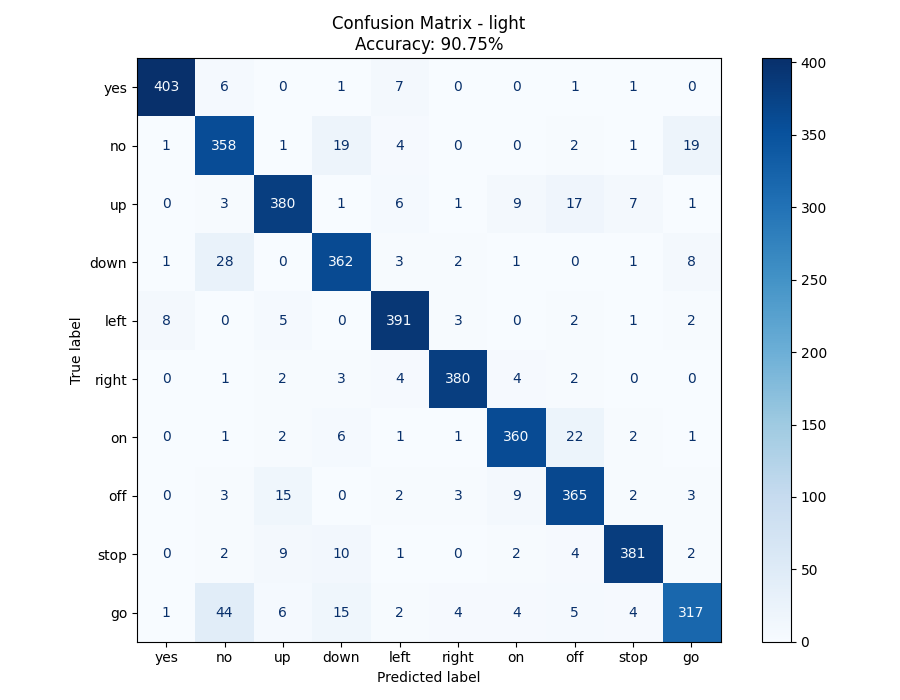
\includegraphics[width=0.7\textwidth]{..//eval_out/confusion_light.png}
    \caption{Matrice di confusione del modello LightCNN.}
    \label{fig:confusion_light}
\end{figure}

La matrice di confusione mostrata in Figura~\ref{fig:confusion_light} evidenzia che il modello leggero riesce a riconoscere correttamente una parte consistente dei comandi, ma mostra ancora errori concentrati tra classi vicine dal punto di vista acustico. In particolare, i comandi brevi e molto simili tra loro tendono a essere scambiati con maggiore frequenza, segnale che la rete cattura bene le strutture più evidenti ma fatica nei casi ambigui.

\subsection{Matrice di confusione del modello ResNet}

\begin{figure}[H]
    \centering
    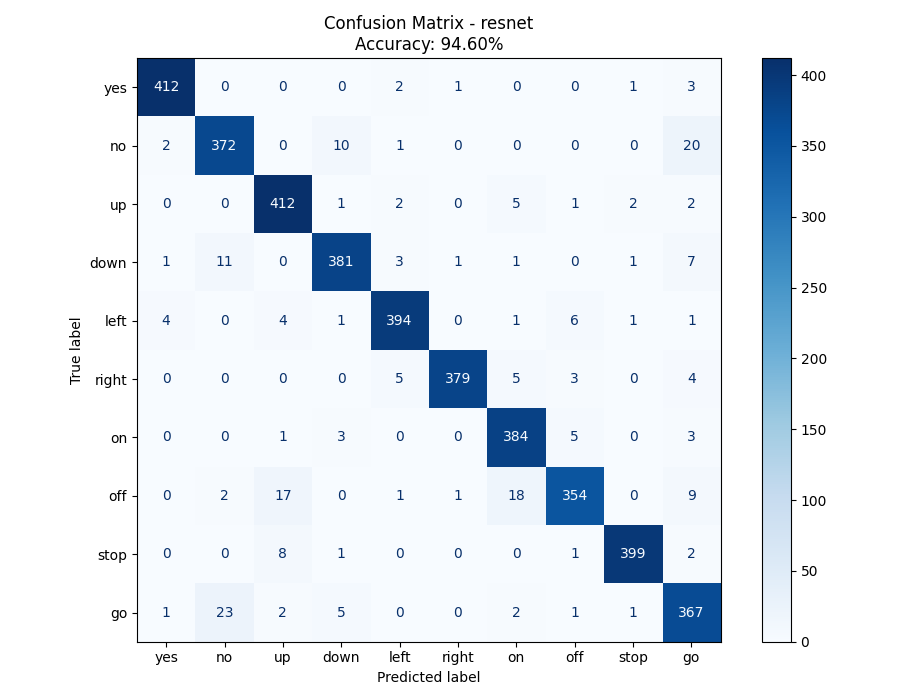
\includegraphics[width=0.7\textwidth]{..//eval_out/confusion_resnet.png}
    \caption{Matrice di confusione del modello AudioResNet.}
    \label{fig:confusion_resnet}
\end{figure}

Rispetto al modello leggero, la ResNet offre una rappresentazione più ricca e in genere produce una separazione più netta tra le classi. La Figura~\ref{fig:confusion_resnet} mostra comunque che anche una rete più profonda non elimina del tutto le confusioni tra comandi simili, soprattutto quando la pronuncia è rapida o il segnale è meno netto. Il vantaggio principale della rete più profonda è una maggiore robustezza generale, mentre il limite rimane la naturale sovrapposizione acustica di alcune parole del dataset.

\subsection{Analisi degli errori}

Per capire meglio il comportamento del classificatore, i campioni errati vengono salvati nella cartella \texttt{eval\_out/wrong\_samples/}. I file CSV \texttt{wrong\_light.csv} e \texttt{wrong\_resnet.csv} permettono di ispezionare le predizioni sbagliate insieme alla confidenza associata alla classe predetta.

Questa analisi mette in evidenza un fenomeno ricorrente: molte delle errate classificazioni riguardano comandi foneticamente vicini oppure pronunciati in modo poco uniforme. Nei risultati osservati emergono errori frequenti tra \texttt{go}, \texttt{no}, \texttt{right}, \texttt{left}, \texttt{up}, \texttt{down}, \texttt{off} e \texttt{stop}. Il comportamento è coerente con la natura del dataset, in cui la variabilità tra parlanti, velocità di pronuncia e qualità della registrazione influisce molto sulla separabilità delle classi.

Questa parte della valutazione è importante anche dal punto di vista della consegna, perché mostra una lettura critica delle prestazioni: un modello può ottenere una buona accuracy complessiva e comunque fallire sistematicamente su alcune classi. Nel contesto del progetto questo aspetto conta più del valore assoluto dell'accuracy, perché dimostra la capacità di interpretare il modello e non soltanto di riportarne il punteggio.

\subsection{Considerazioni sulla scelta del modello}

Dal punto di vista pratico, LightCNN rappresenta una soluzione adatta quando si desidera un sistema semplice, veloce e facilmente addestrabile anche su hardware limitato. AudioResNet, invece, è più indicato quando si cerca una maggiore capacità espressiva e si accetta un costo computazionale superiore. In questo progetto il confronto tra i due approcci mostra bene il classico compromesso tra efficienza e accuratezza: la rete più piccola è più snella, mentre quella più profonda tende a generalizzare meglio sulle configurazioni più difficili.

\section{Conclusioni}

In conclusione, il progetto conferma che il riconoscimento di comandi vocali è un problema naturale per le reti neurali convoluzionali quando l'audio viene trasformato in spettrogrammi Mel. La pipeline implementata è coerente e modulare: il dataset viene filtrato, il test set resta separato dal training, la rappresentazione tempo-frequenza viene costruita in modo uniforme e i modelli vengono valutati sia quantitativamente sia qualitativamente.

I risultati ottenuti mostrano che il sistema è già funzionale, ma lascia spazio a ulteriori miglioramenti. Le direzioni più interessanti riguardano l'augmentation audio, una migliore calibrazione degli iperparametri, l'uso di architetture più sofisticate o di tecniche di ensemble e un'analisi ancora più accurata dei casi errati. In sintesi, la parte decisiva del progetto non è soltanto la scelta del modello, ma il bilanciamento tra preprocessing, complessità della rete, qualità dei dati di input e capacità di interpretare correttamente le prestazioni ottenute.

\end{document}
